\documentclass{article}
\usepackage{amsmath}
\usepackage{mathrsfs}
\usepackage{amssymb}
\usepackage{amsfonts}
\usepackage{gauss}
\usepackage[top=1in,bottom=1in,left=1.25in,right=1.25in]{geometry}
\usepackage{dsfont}
\usepackage{amsthm}
\usepackage{graphicx}
\usepackage{multirow}
\usepackage{textcomp}
\usepackage{bbm}
\usepackage{wasysym}
\usepackage{fancyhdr}
\usepackage{setspace}
\pagestyle{fancy}
\lhead{Instructor: Prof. Hohberger}
\chead{Vv285 Project : Rainbow}
\rhead{SJTU-UM Joint Institute}
\lfoot{}
\cfoot{\thepage}
\rfoot{}



\begin{document}
%\bibliographystyle{plain}
%\bibliography{reference.bib}
\begin{titlepage}
\begin{center}
\includegraphics{logo_1.jpg}\\[1.5cm]

\textsc{\Huge  Vv285 Honors Mathematics III}\\[2cm]

\textsc{\huge  Term Project}\\[1.5cm]

{\huge \bfseries R A I N B O W S}\\[2cm]

\Large \emph{Instructor:}\\
Dr. Horst Hohberger\\[2cm]

\Large \emph{Author:}\\
Li Chunchao	5143709188\\
Jiang Zhang	5143709201\\
Zuo Jiaqi	5143709174\\
Shen Yue	5143709045\\
Han Heming	5143709133

\vfill
{\large \today}
\end{center}
\end{titlepage}
\begin{spacing}{1.5}
\section*{Abstract}
This project focuses on the mathematical interpretation and properties of rainbows. First, we do some research on rainbow and combine the information together with our life experience. Then we use the knowledge from geometry and calculus to help us understand and explain the features of rainbow. We carry out this project to build up a model to analyze the rainbow phenomena, and we aim to use our model to simulate and predict the behavior of rainbow.
\newpage
\tableofcontents
\newpage
\section{Introduction}
\subsection{Rainbow}
Sunshine passes through the spherical water drop in the air after a series of refraction and reflection will create rainbow. Traditionally, the rainbow's colors are described as red, orange, yellow, green, blue, indigo and violet. In fact, our eyes can discern many more individual hues. Sometimes we can observe secondary rainbow, but less often. Higher order rainbow is even rarer.(see figure \ref{rainbow}) In this project, we will analyze the formation and property of the rainbow.\\
\begin{figure}[!htb]
\centering
\includegraphics[width=12cm]{rainbow.jpg}
\caption{Multi-Rainbow. Taken from \cite{Rainbow}}
\label{rainbow}
\end{figure}
\\
The figure above is a rare scene of multi-rainbow.\\
\\
\subsection{Our Project}
The first part of our project is a set of some basic work, such as exploring the angle of deviation, and explaining some natural phenomena including why rainbow appears arched and why rainbow's colors appear at specific position. We also use the background information and knowledge of geometry and calculus to explore the mathematical relationship between physical quantities, and explore the secondary and tertiary rainbow.\\
\\
The second part is some extended exploration. We use the conclusions from previous part and apply them to solve more complicated problems. We also use our programming skills, plot some figures to induce some hypothesis and verify them by mathematical calculation.
\subsection{Basic Knowledge of Optics}
\subsubsection{Snell's Law}
Snell's Law which is also known as the Snell Descartes Law and the Law of Refraction, illustrates the relationship between the angles of incidence and refraction by following formula \cite{Snell's Law}:
\begin{figure}[!htb]
\centering
\includegraphics[width=4cm]{snell.png}
\caption{Snell's Law. Figure taken from \cite{Snell's Law}}
\end{figure}
\\
$$\frac{\sin\theta_1}{\sin\theta _2}=\frac{v_1}{v_2}=\frac{\lambda_1}{\lambda_2}=\frac{n_2}{n_1}$$
This formula is useful not only to light but also other waves when they pass through the boundary between two different isotropic media, such as water-air, glass-water, or air-water. 
Here:\\
\indent $\theta$ is the angle measured from the normal of the boundary to the incidence ray or refraction ray;\\
\indent v is the speed of light in the corresponding medium (m/s);\\
\indent $\lambda$ is the wavelength of light in the corresponding medium;\\
\indent n is the refractive index of the corresponding medium.
\subsubsection{Law of Reflection}
We only discuss specular reflection here.\\
\newpage
Specular reflection is ``the mirror-like reflection of light (or of other kinds of wave) from a surface".
\begin{figure}[!htb]
\centering
\includegraphics[width=4cm]{reflection.png}
\caption{Law of Specular Reflection. Figure taken from \cite{Reflection}}
\end{figure}
\\
Light coming from a single direction is reflected to a single direction. In this process, the direction of i.e. $\theta _i =\theta _r$, and ``the incident, normal, and reflected directions are coplanar". \cite{Reflection}
\newpage
\section{Basic Task}
In this section, we will use basic knowledge of geometry and calculus, as well as common sense of rainbow to solve these questions.
\subsection{Angle of Deviation}
\  \\
\begin{figure}[!htb]
\centering
\includegraphics[width=8cm]{2_1.png}
\caption{Formation of the Primary Rainbow. Figure taken from \cite{Calculus}}
\end{figure}
\\
From the picture, we know that
\begin{align*}
\angle AOC& = 2\angle ABC = 4\beta\\
\angle OAC& =\angle OCA = \frac{1}{2}(\pi - \angle AOC)=\frac{\pi}{2}-2\beta\\
\angle PAO& = \angle PCO = \alpha
\end{align*}
Then, $$\angle PAC=\angle PAO + \angle OAC=\frac{\pi}{2}-2\beta+\alpha$$
$$\angle PCA=\angle PCO +\angle OCA = \frac{\pi}{2}-2\beta +\alpha$$
$$D(\alpha)=\angle PAC + \angle PCA =\pi + 2\alpha -4\beta$$
\subsection{Rainbow Appears Arched}
\label{abc}
According to the Snell's law, $n_1\sin\alpha = n_2\sin\beta$, where $n_1, \ n_2$ are refractive index. As the light travels from vacuum to the spherical water droplet, we can set $n_1=1, \ n_2=n$, where $n$ is a constant. Hence we can get
\begin{align*}
D(\alpha)&=\pi+ 2\alpha -4\beta =\pi +2\alpha - 4\arcsin(\frac{\sin\alpha}{n})\\
D'(\alpha) &= 2 - 4\frac{1}{\sqrt{1-\frac{\sin^2\alpha}{n^2}}}\frac{\cos \alpha}{n}=2-\frac{4\cos \alpha}{\sqrt{n^2-\sin^2\alpha}}
\end{align*}
Assume $D'(\alpha)=0$, then we have \begin{align*}\alpha_0&=\arccos\sqrt{\frac{n^2-1}{3}}\\\delta_0&=D(\alpha_0)=\pi+2\arccos\sqrt{\frac{n^2-1}{3}}-4\arcsin\sqrt{\frac{4}{3n^2}-\frac{1}{3}}
\end{align*}
When light enter the water from the air, the refractive index is $n=1.333$ \cite{Optics}. Plug $n$ into the formula above, we get $\alpha_0 \approx 59.4^{\circ}$, $\delta_0\approx 138^{\circ}$\\
\begin{align*}
rainbow\ angle=180^{\circ}-138^{\circ}=42^{\circ}
\end{align*}\\
\\
Now we will discuss why a rainbow appears as an arc.\\
\\
Rainbow is formed by sunshine passing through the spherical water drop in the air after a series of refraction and reflection. The angles of incidence are different; rays of light after reflection are on different direction. The intensity of light reaches the highest point at some specific angle (about 42$^{\circ}$). Only ray of light in this range gotten by human eyes, the rainbow is visible. As a result, if we take human eyes as a center, and draw an axis paralleled to the direction of the sunlight, then sunlight reaches one’s eyes in a same angle will form a complete circular conical surface about this axis. Hence a rainbow appears as an arc.
\newpage
\subsection{Colors and Positions}
\ \\
\begin{figure}[!htb]
\centering
\includegraphics[width=8cm]{2_3.png}
\caption{Formation of Different Colors}
\end{figure}
\\
Rainbows span a continuous spectrum of colors. Any distinct bands perceived are an artefact of human color vision, and no banding of any type is seen in a black-and-white photo of a rainbow, only a smooth gradation of intensity to a maximum, then fading towards the other side. For colors seen by the human eye, the most commonly cited and remembered sequence is Newton's sevenfold red, orange, yellow, green, blue, indigo and violet.
\subsection{Secondary Rainbow}
\begin{figure}[!htb]
\centering
\includegraphics[width=8cm]{2_4.png}
\caption{Formation of the Secondary Rainbow. Figure taken from \cite{Calculus}}
\end{figure}
From the picture, it is easy to see that \begin{align*}\angle AOB =\angle BOC = \angle COD = \pi -2\beta.\end{align*}
Hence, \begin{align*}
\angle AOD = 2\pi -\angle AOB -\angle BOC -\angle COD = 2\pi -3(\pi -2\pi)=6\beta - \pi.
\end{align*}
Thus,
\begin{align*}
\angle OAD &= \angle ODA = \frac{\pi - \angle AOD}{2} = \pi - 3\beta\\
\angle PAD &= \pi - \angle OAD -\alpha = 3\beta -\alpha\\
\angle PDA &= \pi - \angle ODA - \alpha = 3\beta -\alpha
\end{align*}
So \begin{align*}D(\alpha)=2\pi - \angle PAD - \angle PDA = 2\pi  + 2\alpha - 6\beta.\end{align*}
Assume $\sin \alpha = n \sin \beta$ as we did in $ii)$, then \begin{align*}
D(\alpha)&= 2\pi  + 2\alpha - 6\arcsin(\frac{\sin \alpha }{n})\\
D'(\alpha)&= 2- 6\frac{1}{\sqrt{1-\frac{\sin^2\alpha}{n^2}}}\frac{\cos \alpha}{n}
\end{align*}
Let $D'(\alpha)=0$, we can obtain \begin{align*}\alpha_0&= \arccos \sqrt{\frac{n^2-1}{8}}\\ \delta_0 &= D(\alpha_0)=2\pi + 2\alpha_0 - 6 \arcsin(\frac{\sin \alpha_0}{n}).\end{align*}
From section \ref{abc}, $n= 1.333$. Plug $n$ into the formula above, we obtain \begin{align*}\alpha_0 \approx 71.8^{\circ},  \ \delta_0 = 231^{\circ}\end{align*} 
so that 
\begin{align*}rainbow\ angle=231^{\circ} -180^{\circ}=51^{\circ}\end{align*}
\\
Some of the light rays will be refracted during the first reflection. Some of the light rays will continue being reflected when they are refracted out of the droplets. Besides, its light is spread over its greater angular extent. \cite{Atoptics} Hence the intensity of the secondary rainbow is less than that of the primary rainbow.\\
\\
The order of the colors is reversed comparing to the primary rainbow. Red light is refracted least and so its rays suffer the smallest deviation. But the total deviation is more than 180$^{\circ}$ and the least deviated rays appear at the inside of the bow. The secondary has $43\%$ of the total brightness of the primary \cite{Atoptics}.\\
\\
In seven colors, red light ray has the smallest refract index$(n)$, because it has the smallest wave length. Furthermore, due to the smallest refract index$(n)$, red light ray has the smallest angle of deviation. Analogously, purple light ray has the biggest wave length. That leads to its biggest angle of deviation.\\
\\
We can use the difference between the angles of deviation of red light ray and purple light ray to represent the width of rainbow. Here, the refract index of red light ray is $n_{1}=1.333$ \cite{Optics} and that of purple light ray is $n_{2}=1.340$ \cite{1.340}.\\
\\
From the primary rainbow:\\
\indent \indent The angle of deviation of red light ray is $\theta_{1}=137.9219^{\circ}$.\\
\indent \indent The angle of deviation of purple light ray is $\theta_{2}=138.9290^{\circ}$.\\
\indent \indent The width is $\theta_{2}-\theta_{1}=1.0071^{\circ}$.\\
\\
From the secondary rainbow:\\
\indent \indent The angle of deviation of red light ray is $\varphi_{1}=230.8908^{\circ}$.\\
\indent \indent The angle of deviation of purple light ray $is \varphi_{2}=232.7088^{\circ}$.\\
\indent \indent The width is $\varphi_{2}-\varphi_{1}=1.8180^{\circ}$.\\
\\
Hence the rate is $1.8180/1.0071\approx1.8$. That means the secondary rainbow's width is 1.8 $\times$ width of the primary rainbow.
\subsection{Tertiary Rainbow}
From the picture, we know that \begin{align*}\angle AOB=\angle BOC = \angle COD =\angle DOE = \pi -2 \beta.\end{align*}
\begin{figure}[!htb]
\centering
\includegraphics[width=8cm]{2_5.png}
\caption{Formation of the Tertiary Rainbow.}
\end{figure}
\\
Hence, \begin{align*}\angle AOE &= 2\pi - \angle AOB -\angle BOC -\angle COD - \angle DOE\\&=2\pi- 4(\pi - 2\beta)=8\beta - 2\pi.\end{align*}
Also, \begin{align*}\angle QEO = \pi -\alpha, \ \angle PAO =\pi -\alpha.\end{align*} 
Then \begin{align*}
D(\alpha)&=2\pi - \angle QEO -\angle PAO - \angle AOE +\pi = 3\pi + 2\alpha -8\beta\\
D'(\alpha)&=2-8\frac{1}{\sqrt {1-\frac{\sin^2\alpha}{n^2}}}\frac{\cos \alpha}{n}
\end{align*}
Let $D'(\alpha)=0$, we can obtain 
\begin{align*}\alpha_0&= \arccos \sqrt{\frac{n^2-1}{15}}\\ \delta_0 &= D(\alpha_0)=3\pi + 2\alpha_0 -  8\arcsin(\frac{\sin \alpha_0}{n}).\end{align*}
From section \ref{abc}, $n=1.333$. Plug $n$ into the formula above, we obtain \begin{align*}\alpha _0\approx 76.8^{\circ}, \ \delta_0=318^{\circ}\end{align*} 
so that\begin{align*}rainbow\ angle=360^{\circ} - 318^{\circ}=42^{\circ}\end{align*}.\\
\\
Some of the light rays will be refracted during the second reflection. Some of the light rays will continue being reflected when they are refracted out of the droplets.\\
\\
The order of the colors is the same as the primary rainbow. Red light is refracted least and so its rays suffer the smallest deviation and the total deviation of the red light in the tertiary rainbow is more than 180$^{\circ}$, which is the same as the secondary rainbow. However, unlike the secondary rainbow, the tertiary rainbow appears sunwards and centered on the sun. \cite{Atoptics} That means the order is reversed comparing to the secondary rainbow, that is, that same as the primary rainbow.\\
\\
We can use the same way and data in the previous section to analyze the tertiary rainbow:\\
\indent \indent The angle of deviation of red light ray is $\phi_{1}=318.2627^{\circ}$.\\
\indent \indent The angle of deviation of purple light ray is $\phi_{2}=320.8146^{\circ}$.\\
\indent \indent The width is $\phi_{2}-\phi_{1}=2.5519^{\circ}$.\\
\\
Hence, the rate is $2.5519/1.0071\approx 2.5$. That means the width of the tertiary rainbow is 2.5 $\times$ width of the primary rainbow.


\section{Project Extension}
In this part, we use the conclusions from the previous part and do some extending exploration.
\subsection{Density of Light Rays}
(a)When $D'(\alpha)\neq 0$, by L'Hospital principle, we have
$$\underset{\varepsilon\rightarrow 0}{\lim}\rho(J'_{\varepsilon})=\frac{2}{D'(\alpha_0)-(-D'(\alpha_0))}=\frac{1}{D'(\alpha_0)}$$
If there exists a $J_{\varepsilon '}$ such that $D:J_{\varepsilon '}\rightarrow I_{\varepsilon}$ is surjective, fix $\varepsilon$, when $D'(\alpha)=0$, by definnition we know that 
$$D(a_0+\varepsilon_0)=D(\alpha_0)+o(\varepsilon')$$
Since $|\frac{o(\varepsilon ')}{\varepsilon '}|\rightarrow 0$, we can let $-\frac{\varepsilon}{2}<\frac{o(\varepsilon ')}{\varepsilon '}<\frac{\varepsilon}{2}$, then we can hence yield 
$$-\frac{\varepsilon\varepsilon '}{2}<o(\varepsilon ')<\frac{\varepsilon\varepsilon '}{2}$$
Meanwhile, since $\varepsilon'\rightarrow 0\Rightarrow \varepsilon '<1$.\\
We can hence yield:
$$-\frac{\varepsilon}{2}<-\frac{\varepsilon\varepsilon '}{2}<o(\varepsilon ')<\frac{\varepsilon\varepsilon '}{2}<\frac{\varepsilon}{2}$$
Thus $$D(\alpha_0+\varepsilon_0)=D(\alpha_0)+o(\varepsilon ')\in(D(\alpha_0)-\frac{\varepsilon}{2},D(\alpha_0)+\frac{\varepsilon}{2})$$
Since $D:J_{\varepsilon '}\rightarrow I_{\varepsilon}$ is surjective,\\
$D(\alpha_0)\in[\delta_0-\varepsilon,\delta_0+\varepsilon]$ no matter what value $D(\alpha_0)$ takes.\\
We know that
$$I_{\epsilon_0}=(D(\alpha_0)-\frac{\varepsilon}{2},D(\alpha_0)+\frac{\varepsilon}{2})\neq[\delta_0-\varepsilon,\delta_0+\varepsilon]$$
Thus $J_{\varepsilon '}$ can't be surjective.\\
\\
(b)When $D'(\alpha)=0$, $$\rho(J'_{\varepsilon})=\frac{2\varepsilon '}{o(\varepsilon ')}=\infty$$
Hence the density of the light ray becomes infinite when $D'(\alpha)=0$.

\subsection{Different Region's Lightness}
From former research, we have:
\begin{align*}
\varrho(\alpha)=\frac{1}{D'(\alpha)}
\end{align*}
Thus only when $D'(\alpha)\geq0\Rightarrow \varrho(\alpha)>0$, the light could reach human's eyes.\\
\begin{figure}[!htb]
\centering
\includegraphics[width=8cm]{8.png}
\caption{Light Path to Human Eyes.}
\end{figure}
\\
\newpage
\ \\
Since the angle of deviation: $D(\alpha)=\pi+2\alpha-4\beta$.\\
We know that: 
\begin{align*}
&D'(\alpha)=2-\frac{4\cos\alpha}{\sqrt{n^2-\sin^2\alpha}}\ \\
&D''(\alpha)=\frac{4(n^2-1)\sin\alpha}{(n^2-\sin^2\alpha)^{\frac{3}{2}}}
\end{align*}
Since $\alpha\in(0,\frac{\pi}{2})$ and $n>1\Rightarrow (n^2-1)\sin\alpha>0$ and $n^2-\sin^2\alpha>n^2-1>0\Rightarrow D''(\alpha)>0$.\\
Notice that the rainbow angle $\theta$ satisfies $\theta(\alpha)=\pi-D(\alpha)=4\beta-2\alpha$. Hence 
\begin{align*}
&\theta'(\alpha)=-D'(a)\\&\theta''(\alpha)=-D''(\alpha)<0
\end{align*}
From the former research we know that $\alpha_0=\arccos\sqrt{\frac{n^2-1}{3}}$ and that $D'(\alpha_0)=0.$\\
Thus we know that $\theta(\alpha_0)$ is the maximum angle and only when $\theta(\alpha)\le\theta(\alpha_0)$, we have $$D'(\alpha)\geq 0$$
Recall that the area of rainbow is the area that $D'(\alpha)=0$ for n of all kinds of visible light.\\
Therefore for the region under the rainbow we have $D'(\alpha)>0$, which means all kinds of visible light could reach human's eye from the droplets below the rainbow by refraction.\\
Thus the region under a rainbow is lighter than that outside the rainbow.\\
Similarly, we know that for the region between the primary and the secondary rainbow, \\
$D'(\alpha)<0$, which means no visible lights could reach human's eyes from the droplets in this area by refraction.\\
Therefore the region between the primary and the secondary rainbow is darker.

\subsection{kth Order Formula}
We denote the total angle which the light has travelled by $D(\alpha)$.\\
When the light is refracted from the vacuum to the spherical water droplet, it turns $\alpha - \beta$ (Figure \ref{f1}).\\
\begin{figure}[!htb]
\centering
\includegraphics[width=8cm]{4.png}
\caption{Refraction From the Vacuum to the Spherical Water Droplet.}
\label{f1}
\end{figure}
\\
\newpage
\ \\
\begin{figure}[!htb]
\centering
\includegraphics[width=8cm]{5.png}
\caption{Refraction From the Spherical Water Droplet to the Vacuum.}
\label{f2}
\end{figure}
\\
Similarly, when the light is refracted from the water droplet to the vacuum, it also turns $\alpha - \beta$ (Figure \ref{f2}).\\
When the light is reflected in the water droplet, it turns $\pi-2\beta$ after one reflection (Figure \ref{f3}).\\
\begin{figure}[!htb]
\centering
\includegraphics[width=8cm]{6.png}
\caption{Reflection in the water droplet.}
\label{f3}
\end{figure}
\\
It is easy to see the light turns in the same direction (clockwise in the previous figures). We can conclude that the total angle of deviation for the $k$th order rainbow is \begin{align*}
D(\alpha) = \alpha - \beta + k(\pi - 2\beta )+\alpha - \beta = k\pi +2\alpha-(2k+2)\beta
\end{align*}
From the previous part, $\sin \alpha = n \sin \beta$. Hence we get \begin{align*}
D(\alpha) &= k\pi +2\alpha-(2k+2)\arcsin(\frac{\sin\alpha}{n})\\
D'(\alpha) &= 2 - (2k+2)\frac{1}{\sqrt{1-\frac{\sin^2\alpha}{n^2}}}\frac{\cos \alpha}{n}
\end{align*}
If we set $D'(\alpha)=0$, then we can obtain \begin{align*}
&\alpha_0(k)=\arccos\sqrt\frac{n^2-1}{k^2+2k}\\
&\delta_0(k)=D(\alpha_0(k))= k\pi + 2\arccos\sqrt\frac{n^2-1}{k^2+2k} - (2k+2)\arcsin(\frac{1}{n}\sqrt{\frac{(k+1)^2-n^2}{k^2+2k}})
\end{align*}
for the $k$th order rainbow, where $n=1.333$ \cite{Optics}.
\\
\\
Next, we draw the graph of $\delta_0(k)-k. \ (1\leq k\leq 20, \ k\in \mathbb{N})$\\
\begin{figure}[!htb]
\centering
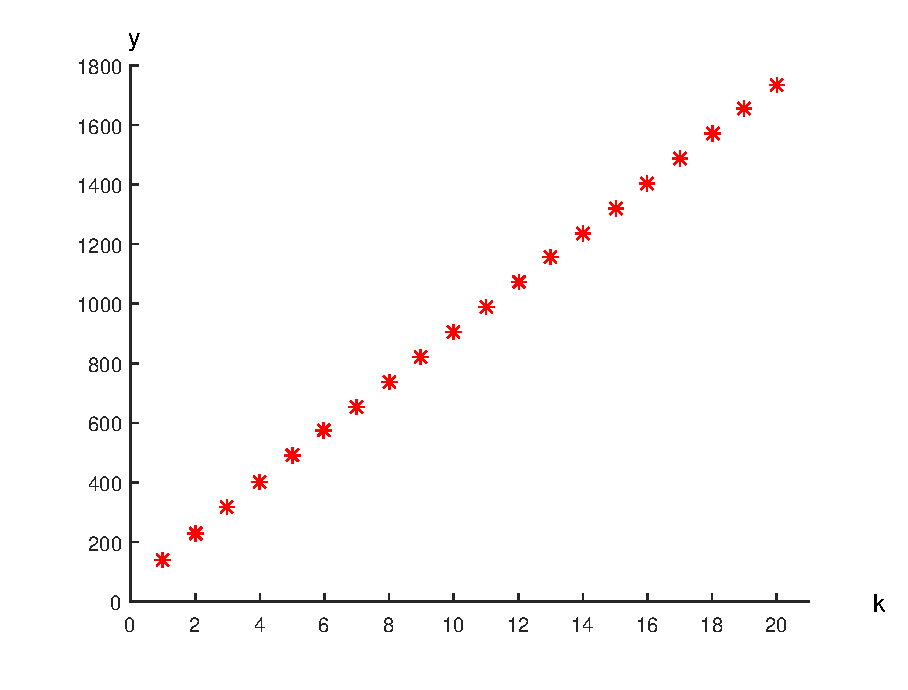
\includegraphics[width=10cm]{Figure1.eps}
\caption{The Graph of $\delta_0(k)-k$}
\label{1}
\end{figure}\\
Now, we will judge the order of seven colors for the $k$th rainbow and find the rainbow angle.\\ 
First, we need to put $\delta_0(k)$ into the interval $[0,2\pi]$. We can assume \begin{align*}2t\pi \leq \delta_0(k)\leq 2(t+1)\pi, \ t\in\mathbb{N}\end{align*}
Then we set \begin{align*}
f(k)=\delta_0(k)-2t\pi, \ t\in\mathbb{N}
\end{align*}
It is easy to see $f(k)\in[0,2\pi]$.\\
Let's see the graph of $f(k)$ \\
\begin{figure}[!htb]
\centering
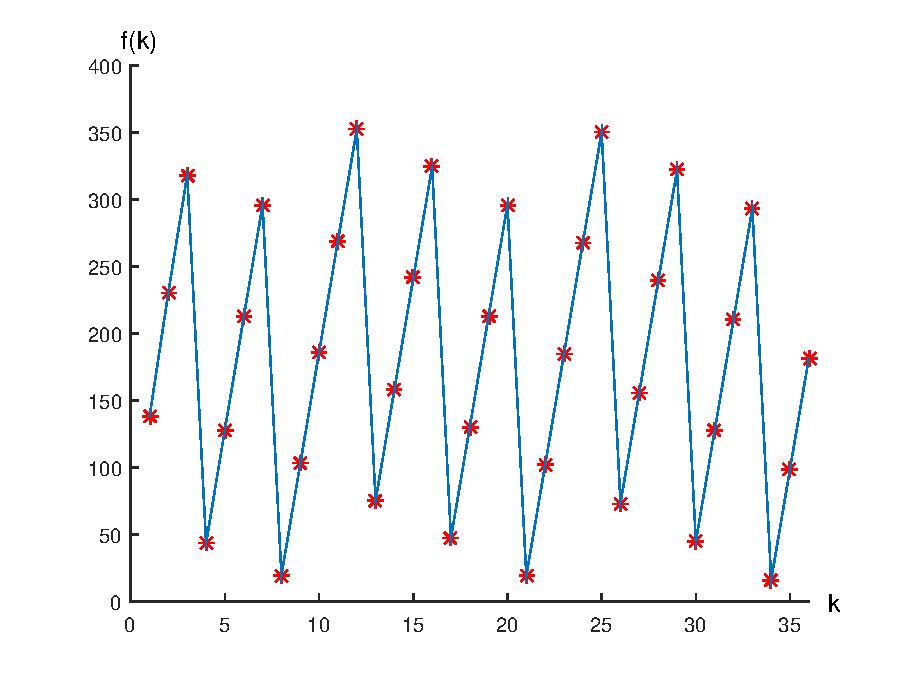
\includegraphics[width=10cm]{Figure2.eps}
\caption{The Graph of $f(k)$}
\end{figure}
\\
It seems that $k$ has a special relationship with $t$.\\
From the graph, we summary that \begin{align*}
t=3[\frac{k-1}{13}]+d
\end{align*}
where $[x]$ represents the greatest integer that is not larger than $x$ and
\begin{equation*}
d=
\begin{cases}
0\quad & 0\leq k\mod 13\ \leq 3\\
1 \quad& 4\leq k\mod 13\ \leq 7\\
2 \quad & 8\leq k\mod 13\ \leq 12
\end{cases}
\end{equation*}
Hence we can get \begin{align*}
f(k)= \delta_0(k)-2\cdot(3[\frac{k-1}{13}]+d)\pi
\end{align*}
We will use $f(k)$ to judge the order of seven colors for the $k$th rainbow and we obtain a criterion.\\\\
\textbf{Criterion}: \\
\indent \indent If $f(k)\in[0,\pi]$, then the $k$th order rainbow has the same color-sequence with the primary rainbow.\\
\indent \indent If $f(k)\in[\pi,2\pi]$, then the $k$th order rainbow has the reversed color-sequence comparing to the primary rainbow.\\
\\
This criterion is intuitively reasonable and easy to check from the secondary and tertiary rainbow.\\
Then we will find a method to calculate the rainbow angle. First, we need to put $\delta_0(k)$ into the interval $[0,\pi]$. We can assume $t\pi\leq \delta_0(k)\leq (t+1)\pi$, $t\in\mathbb{N}$, then we can get $g(k)=\delta_0(k)-t\pi$, $t\in\mathbb{N}$. It is easy to see $g(k)\in[0,\pi]$.\\
\\
Let's see the graph of $g(k)$. \\
\begin{figure}[!htb]
\centering
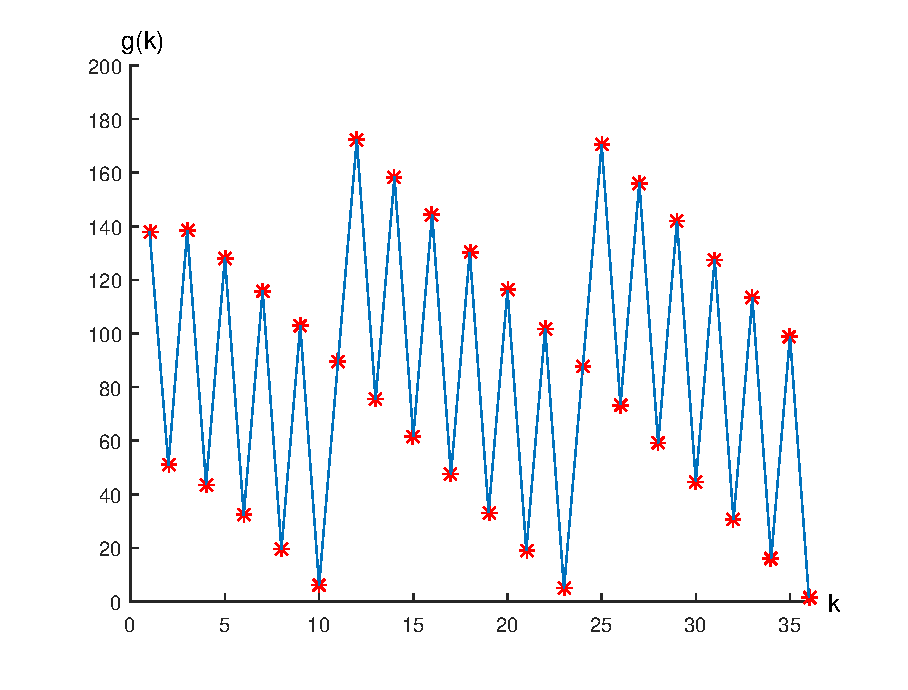
\includegraphics[width=10cm]{Figure3.eps}
\caption{The Graph of $g(k)$}
\end{figure}
\\
However, it is hard to find the specific relationship between $k$ and $t$. So we keep this formula and give the method without proof.\\
Namely, we give the relationship between rainbow angle and $k$:\\
\begin{align*}
Rainbow\ angle=\min\{g(k),180^{\circ}-g(k)\}.
\end{align*}
\ \\
Take $12$th order of rainbow for instance.\\
When $k=12$:\begin{align*} \delta_0(k)=1072.3^{\circ}\end{align*}
The corresponding $f(k)=352.3^{\circ}$ and $g(k)=172.3^{\circ}$.\\
As $f(k)\in[\pi,2\pi]$, the $12$th order rainbow has the reversed order comparing to the primary rainbow.\\
\begin{align*} rainbow\ angle=180^{\circ}-172.3^{\circ}=7.7^{\circ}\end{align*}
\\
Let's see Figure \ref{1} again. It is surprising to see that the graph turns out to be nearly a straight line.\\
\begin{figure}[!htb]
\centering
\includegraphics[width=10cm]{Figure4.eps}
\caption{The Graph of $\delta_0(k)-k$}
\end{figure}
\\
Then, we consider the previous 20 groups of data as a sample. Applying the corresponding knowledge of linear regression, we can obtain the relative equation of linear regression: \begin{align*}\tilde{\delta_0}(k)=83.6258k + 67.1133 \ \ (k\in \mathbb{N})\end{align*}
and the correlation coefficient \begin{align*}
R=0.999969
\end{align*}
\begin{figure}[!htb]
\centering
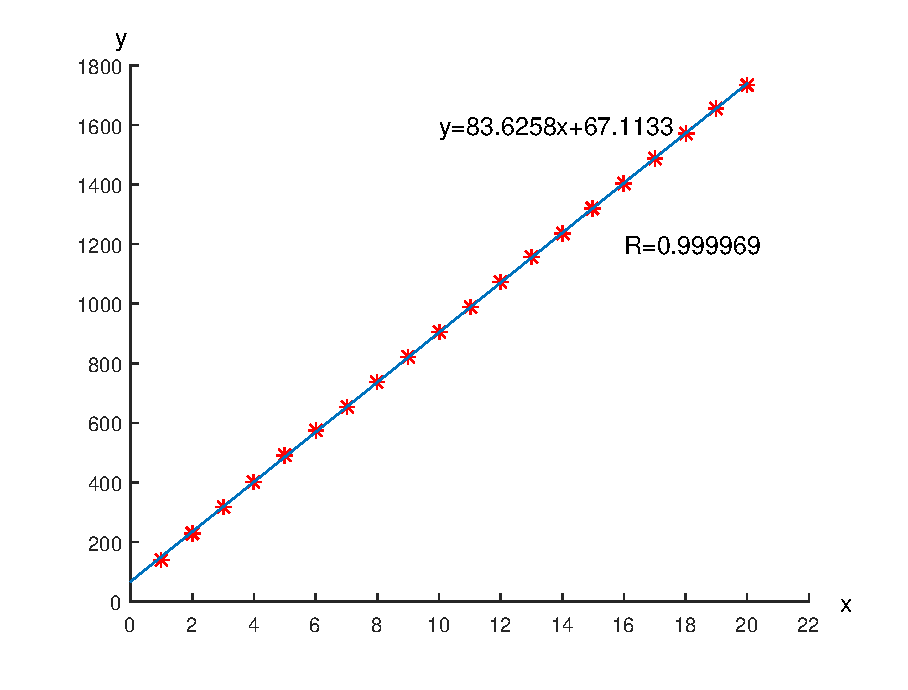
\includegraphics[width=10cm]{Figure5.eps}
\caption{The Graph of $\delta_0(k)-k$}
\end{figure}
\\
After that, we will use this linear approximation to judge the order of the seven colors and find the rainbow angle.\\
\\
i) Order: because of the periodicity, we will first put $\tilde{\delta_0}(k)$ into the interval $[0,2\pi]$.\\
Assume $\tilde{f}(k)=\tilde{\delta_0}(k)-2t\pi$, and $2\pi t\leq \tilde{\delta_0}(k)\leq 2\pi (t+1)$ \quad$(t\in\mathbb{N})$, then\begin{align*}
360t\leq 83.6258k&+67.1133\leq 360(t+1)\\
\Rightarrow \qquad\frac{k-3.5023}{4.3049}\leq &t \leq \frac{k+0.8025}{4.3049}
\end{align*}
As $t\in\mathbb{N}$, we get \begin{align*}
t=[\frac{k+0.8025}{4.3049}]
\end{align*}
where $[x]$ represents the greatest integer that is not larger than $x$.\\
Then 
$$\tilde{f}(k)=83.6258k + 67.1133 - 360[\frac{k+0.8025}{4.3049}], \ k\in \mathbb{N}$$
Using $\tilde{f}(k)$, we can achieve a similar criterion with the previous one to judge the order of the seven colors.\\\\
\textbf{Criterion}: \\
\indent \indent If $\tilde{f}(k)\in[0,\pi]$, then the $k$th order rainbow has the same color-sequence with the primary rainbow.\\
\indent \indent If $\tilde{f}(k)\in[\pi,2\pi]$, then the $k$th order rainbow has the reversed color-sequence comparing to the primary rainbow.\\
\\
This criterion is also intuitively reasonable and easy to check from the secondary and tertiary rainbow.\\
\begin{figure}[!htb]
\centering
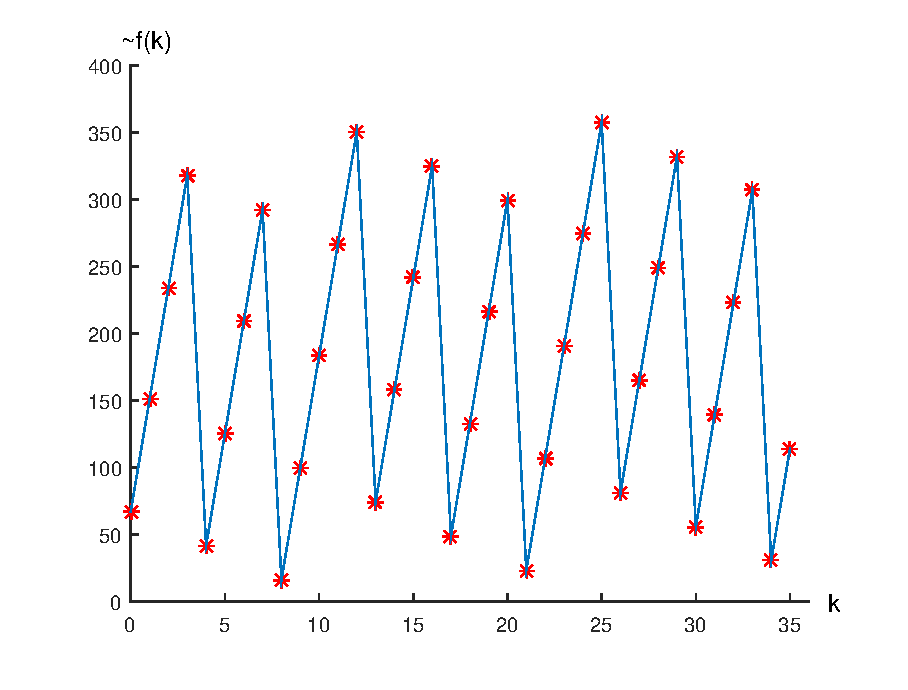
\includegraphics[width=10cm]{Figure6.eps}
\caption{The Graph of $\tilde{f}(k)-k$}
\end{figure}
\\

ii) Rainbow Angle: we will give a method to find the rainbow angle without proof.\\
First, we need to put $\tilde{\delta_0}(k)$ into the interval $[0,\pi]$\\
Assume $t\pi\leq \tilde{\delta_0}(k)\leq (t+1)\pi$, $\tilde{g}(k)=\tilde{\delta_0}(k)-t\pi$, $t\in\mathbb{N}$ then \begin{align*}
180t\leq 83.6258k&+67.1133\leq 180(t+1)\\
\Rightarrow \qquad\frac{k-1.3498}{2.1524}\leq &t \leq \frac{k+0.8025}{2.1524}
\end{align*}
As $t\in\mathbb{N}$, we get \begin{align*}
t=[\frac{k+0.8025}{2.1524}]
\end{align*}
where $[x]$ represents the greatest integer that is not larger than $x$.\\
Also,
\begin{align*}
\tilde{g}(k)=83.6258k+67.1133-180[\frac{k+0.8025}{2.1524}], \ \ k\in\mathbb{N}
\end{align*}
Then \begin{align*}
rainbow\ angle=\min\{\tilde{g}(k),180^{\circ}-\tilde{g}(k)\}
\end{align*}
\begin{figure}[!htb]
\centering
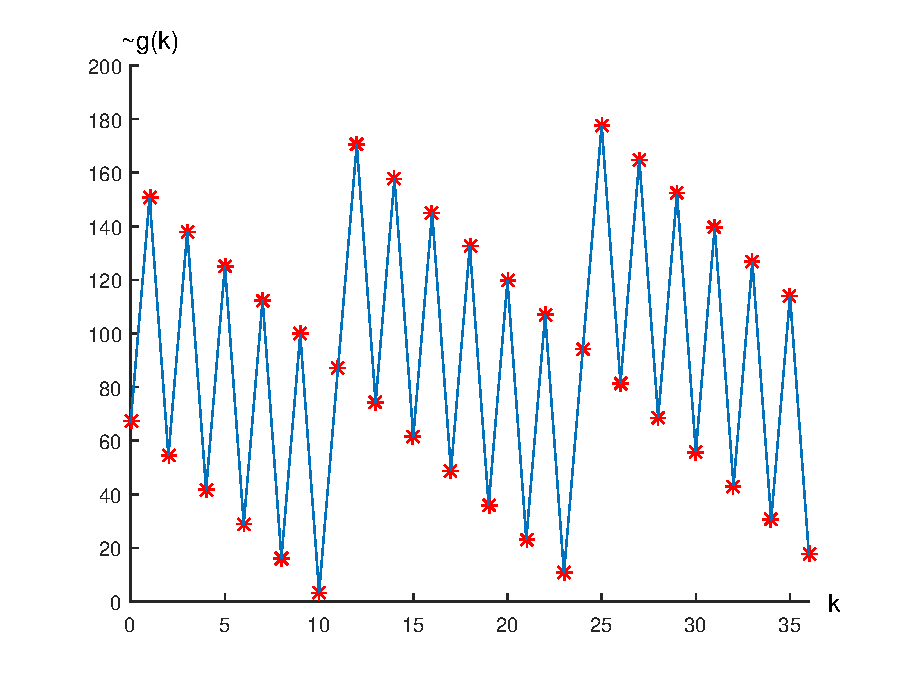
\includegraphics[width=10cm]{Figure7.eps}
\caption{The Graph of $\tilde{g}(k)-k$}
\end{figure}
\\
Again we use the $12$th order rainbow for instance. \\
When $k=12$:
$$\tilde{\delta_0}(k)=1070.6^{\circ}$$
the corresponding
\begin{align*}&\tilde{f}(k)=350.6^{\circ}\\
&\tilde{g}(k)=170.6^{\circ}\end{align*}
As $\tilde{f}(k)\in [\pi,2\pi]$, the $12$th order rainbow has the reversed order comparing to the primary rainbow.\\
Then \begin{align*}
rainbow\ angle=\min\{180^{\circ}-170.6^{\circ},170.6^{\circ}\}=8.4^{\circ} 
\end{align*}
This result coincides with the previous one exactly.\\
\\
Obviously, if we use $\tilde{\delta_0}(k)$, it will be much easier for us to deal with $k$th order rainbow. However, we note that if $k$ is too large, we need to use a larger sample size to make our approximation more accurate.
\subsection{Glory Scattering}
Most of the sunlight entering raindrops leaves the other side without internal reflection. Only a small fraction is reflected to form the primary, secondary and higher order rainbows. These rainbow forming rays are usually very faint. \cite{Atoptics}\\
\\
Now, let’s analyze the diagram of the zero order rainbows.\\
\begin{figure}[!htb]
\centering
\includegraphics[width=8cm]{7.png}
\caption{Zero order rainbow.}
\end{figure}
\\
From the picture, we know that $\angle OAC=\angle OBC=\alpha-\beta$. Then $D(\alpha)= \angle OAC+\angle OBC=2(\alpha-\beta)$. $D’(\alpha)=2>0$, $\alpha\in(0,\frac{\pi}{2})$. That means $D(\alpha)$ does not have a minimum and the outgoing ray deviation increases continuously . There is no turning point or angle of minimum deviation at each side of which the deflection changes in the same direction. This is why the zero order rays do not produce a rainbow. \cite{Atoptics}\\
\\
Although refraction disperses the colors, they overlap again outside the drop. The glow is the same color as the incident sunlight and we can’t see color bands in the glory. \cite{Atoptics}\\
\\
The brightness of the zero order glow is one of the causes of the difficulty in ever seeing 3rd and 4th order rainbows outdoors. \cite{Atoptics}
\newpage
\section{Conclusion and Summary}
In this project, we have deeply discussed and analyzed “the calculus of rainbows”. Starting from basic knowledge of reflection and refraction of light, we discuss the formation of primary rainbow and extend to secondary and tertiary rainbow.\\
\\
In the basic-task part, we first introduce angle of deviation and rainbow angle. This two technical terms turn out to be very important and useful when we are describing the features of rainbow. For example, when we are discussing the color sequence of the rainbow, the angle of deviation and the rainbow angle can be extremely useful to determine this sequence. Besides, we have collected lots of information from Internet to give an explanation to some questions such as “Why is the intensity of the secondary rainbow less than that of the primary rainbow”.\\
\\
The extension of the previous tasks shows a deeper analysis for the topic. Basically, it covers the discussion of the parallel light rays from the sun. Also, we spend lots of pages to investigate the kth order rainbow and we find numerous interesting phenomena when we are doing this part. Besides, we collect lots of data and use linear regression to generate a criterion to determine the color sequence of the rainbow and the rainbow angle. In fact, we compare the result from our method with the theoretical value and the error turns out to be less than 0.1\%. We believe that it will be very useful if we realize this method through computer.\\
\\
We may continue our discussion on this project through the following aspects such as exploring the fact that the light rays are actually not only reflected and refracted but also scattered and diffracted to some extent. Some relative information is included in \cite{Atoptics}.

\end{spacing}
\newpage
\begin{spacing}{2.0}
\begin{thebibliography}{0}
\bibitem[1]{Atoptics}
L. Cowley. Atmospheric optics. http://www.atoptics.co.uk, 2015. Web. Accessed July 25th, 2015.
\bibitem[2]{Calculus}
J. Stewart. \emph{Calculus}. Higher Education Press, 5 edition, 2003.
\bibitem[3]{Optics}
A. Zajac and E. Hecht. \emph{Optics}. Pearson Higher Education, 4 edition, 2003.
\bibitem[4]{Rainbow}
T. Nordvik. Six Rainbows Across Norway. http://apod.nasa.gov/apod/ap070912.html, 2007. Sep. Accessed July 28th, 2015. 
\bibitem[5]{1.340}
M. Abramowitz et al. Refraction of Light. http://micro.magnet.fsu.edu/optics/lightandcolor/refraction.html, 2003. Aug. Accessed July 28th, 2015.
\bibitem[6]{Snell's Law}
Wikipedia. Snell's law — wikipedia, the free encyclopedia, 2015. Web.
Accessed July 29th, 2015.
\bibitem[7]{Reflection}
Wikipedia. Specular reflection — wikipedia, the free encyclopedia, 2015. Web.
Accessed July 29th, 2015.


\end{thebibliography}
\end{spacing}
\end{document}
